% This file was converted to LaTeX by Writer2LaTeX ver. 1.0.2
% see http://writer2latex.sourceforge.net for more info
\documentclass[twoside,letterpaper]{article}
\usepackage[latin1]{inputenc}
\usepackage[T1]{fontenc}
\usepackage[english]{babel}
\usepackage{amsmath}
\usepackage{amssymb,amsfonts,textcomp}
\usepackage{color}
\usepackage{array}
\usepackage{supertabular}
\usepackage{hhline}
\usepackage{hyperref}
\usepackage{cite}
\usepackage{etoolbox}
\ifx\pdftexversion\undefined
\usepackage[dvips]{graphicx}
\else
\usepackage[pdftex]{graphicx}
\DeclareGraphicsRule{*}{mps}{*}{}
\fi

\patchcmd{\thebibliography}{\section*{\refname}}{}{}{}
\hypersetup{pdftex, colorlinks=true, linkcolor=blue, citecolor=blue, filecolor=blue, urlcolor=blue, pdftitle=SYSTEMS REQUIREMENT SPECIFICATION, pdfauthor=Clinton Jeffery, pdfsubject=, pdfkeywords=}
\usepackage[pdftex]{graphicx}
% Outline numbering
\setcounter{secnumdepth}{5}
\renewcommand\thesection{\arabic{section}}
\renewcommand\thesubsection{\arabic{section}.\arabic{subsection}}
\renewcommand\thesubsubsection{\arabic{section}.\arabic{subsection}.\arabic{subsubsection}}
\renewcommand\theparagraph{\arabic{section}.\arabic{subsection}.\arabic{subsubsection}.\arabic{paragraph}}
\renewcommand\thesubparagraph{\arabic{section}.\arabic{subsection}.\arabic{subsubsection}.\arabic{paragraph}.\arabic{subparagraph}}
\makeatletter
\newcommand\arraybslash{\let\\\@arraycr}
\makeatother
% Page layout (geometry)
\setlength\voffset{-1in}
\setlength\hoffset{-1in}
\setlength\topmargin{0.5in}
\setlength\oddsidemargin{1in}
\setlength\evensidemargin{1in}
\setlength\textheight{8.278in}
\setlength\textwidth{6.5in}
\setlength\footskip{0.561in}
\setlength\headheight{0.5in}
\setlength\headsep{0.461in}
% Footnote rule
\setlength{\skip\footins}{0.0469in}
\renewcommand\footnoterule{\vspace*{-0.0071in}\setlength\leftskip{0pt}\setlength\rightskip{0pt plus 1fil}\noindent\textcolor{black}{\rule{0.25\columnwidth}{0.0071in}}\vspace*{0.0398in}}
% Pages styles
\makeatletter
\newcommand\ps@Standard{
  % \renewcommand\@oddhead{\selectlanguage{english}\rmfamily\color{black} College Of Engineering, Trivandrum\hfill \hfill Project SRS}
  % \renewcommand\@evenhead{\@oddhead}
  % \renewcommand\@oddfoot{\foreignlanguage{english}{\textcolor{black}{SRS }}\foreignlanguage{english}{\textcolor{black}{\thepage{}}}}
  % \renewcommand\@evenfoot{\@oddfoot}
  \renewcommand\thepage{\roman{page}}
}
\newcommand\ps@FirstPage{
  \renewcommand\@oddhead{}
  \renewcommand\@evenhead{\@oddhead}
  \renewcommand\@oddfoot{}
  \renewcommand\@evenfoot{\@oddfoot}
  \renewcommand\thepage{\arabic{page}}
}
\makeatother
\pagestyle{Standard}
\setlength\tabcolsep{1mm}
\renewcommand\arraystretch{1.3}
% footnotes configuration
\makeatletter
\renewcommand\thefootnote{\arabic{footnote}}
\makeatother
\title{INTERIM REPORT}
\author{Kevin Joseph, Jayadeep K M, Mohammed. Nisham}
\date{\today}
\begin{document}

\clearpage{\centering\selectlanguage{english}\bfseries\color{black}
INTERIM REPORT   
\par}


\bigskip

{\centering\selectlanguage{english}\bfseries\color{black}
Decision making using Reinforced Deep Learning
\par}


\bigskip

\centering

\includegraphics[width=3cm]{images/logo.jpg}

\bigskip

{\centering\selectlanguage{english}\bfseries\color{black}
\today
\par}


\bigskip


\bigskip

\bigskip

{\centering\selectlanguage{english}\bfseries\color{black}
Prepared by:
\par}

{\centering\selectlanguage{english}\color{black}
Kevin Joseph, Jayadeep K M, Mohammed Nisham K
\par}
\bigskip
{\centering\selectlanguage{english}\bfseries\color{black}
Guide:
\par}

{\centering\selectlanguage{english}\color{black}
Vipin Vasu\\
vipin@cet.ac.in\\
\par}
\bigskip
{\centering\selectlanguage{english}\bfseries\color{black}
College Of Engineering, Trivandrum
\par}

\clearpage{\centering\selectlanguage{english}\bfseries\color{black}
\par}

\bigskip

\setcounter{tocdepth}{9}
\renewcommand\contentsname{}
% \tableofcontents

\bigskip
\flushleft
\setcounter{page}{1}
\pagenumbering{arabic}
\section{Progress}
    \begin{enumerate}
      \item Implemented Q Learning with Tic Tac Toe to understand Q Learning
      \item Researched speed differences and math library performances in java and python for machine learning applications. Fixed python due to abundance of easily accessible deep net libraries, and ale interface.
      \item Researched related projects and associated libraries to be used in project:
      \begin{enumerate}
        \item Associated Libraries
        \begin{enumerate}
          \item Atari Learning Environment
          \item Numpy
          \item Neon
        \end{enumerate}
      \end{enumerate}
      
      \begin{enumerate}
        \item Related Project
        \begin{enumerate}
          \item Deep Mind
          \item Convnet.js
        \end{enumerate}
      \end{enumerate}
    \item Interfaced ALE(4 games) with a random agent.
    \item Interfaced online statistics with agent to plot reward and q function
    \item Created class structure for project.
    \item Created design for agent neural net.
    \end{enumerate}

\newpage
\section{Class Design}
\begin{figure}[ht]
  \centering
  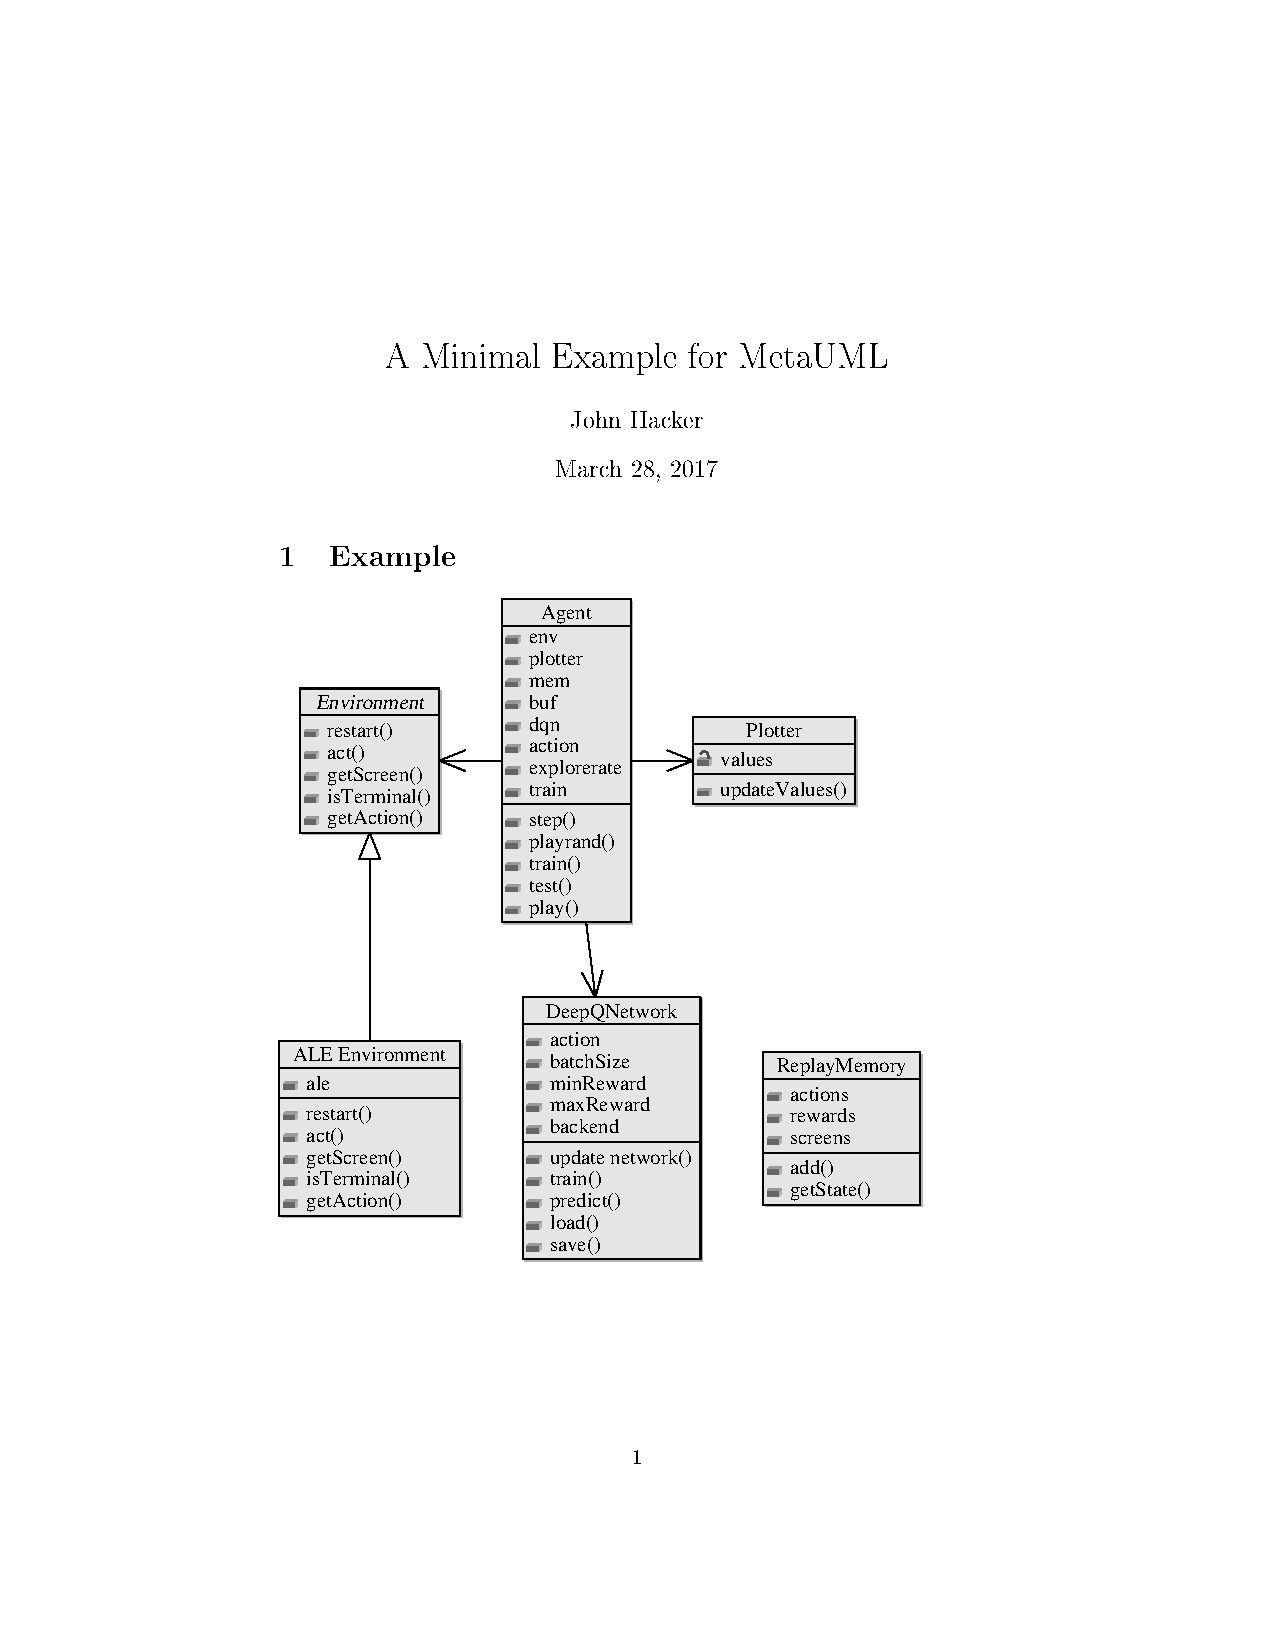
\includegraphics{../../uml/uml.1}
  \caption{Class UML Diagram}
\end{figure}

\newpage
\section{Neural Net Design}
\begin{figure}[ht]
  \centering
  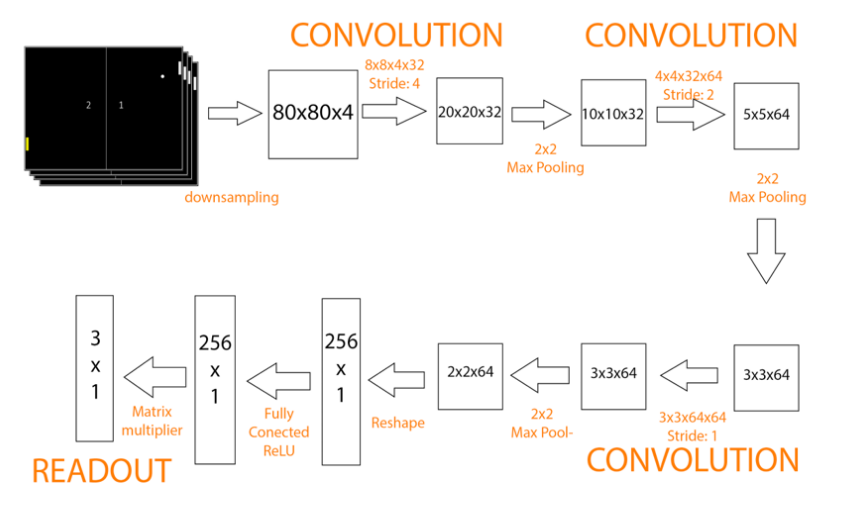
\includegraphics[width=15cm]{images/network}
  \caption{Neural Network Design}
\end{figure}

\newpage
\section{TODO}
\begin{center}
 \begin{tabular}{|c c c|} 
 \hline
 \textbf{\#} & \textbf{Task} & \textbf{Estimated Time} \\ [0.5ex] 
 \hline\hline
 1 & Coding of Intelligent Agent & 2 weeks (In progress)\\ 
 \hline
 2 & Training and testing of Agent & 1 week (depends on gpu) \\
 \hline
\end{tabular}
\end{center}
\end{document}
